\documentclass[a4paper,14pt]{extreport}
\usepackage[left=1.5cm,right=1.5cm,
    top=1.5cm,bottom=2cm,bindingoffset=0cm]{geometry}
\usepackage{scrextend}
\usepackage[T1,T2A]{fontenc}
\usepackage[utf8]{inputenc}
\usepackage[english,russian,ukrainian]{babel}
\usepackage{tabularx}
\usepackage{amssymb}
\usepackage{color}
\usepackage{amsmath}
\usepackage{mathrsfs}
\usepackage{listings}
\usepackage{graphicx}
\graphicspath{ {./images/} }
\usepackage{lipsum}
\usepackage{xcolor}
\usepackage{hyperref}
\usepackage{tcolorbox}
\usepackage{tikz}
\usepackage[framemethod=TikZ]{mdframed}
\usepackage{wrapfig,boxedminipage,lipsum}
\mdfdefinestyle{MyFrame}{%
linecolor=blue,outerlinewidth=2pt,roundcorner=20pt,innertopmargin=\baselineskip,innerbottommargin=\baselineskip,innerrightmargin=20pt,innerleftmargin=20pt,backgroundcolor=gray!50!white}
 \usepackage{csvsimple}
 \usepackage{supertabular}
\usepackage{pdflscape}
\usepackage{fancyvrb}
%\usepackage{comment}
\definecolor{ggreen}{rgb}{0.4,1,0}
\definecolor{rred}{rgb}{1,0.1,0.1}
\usepackage{array,tabularx}
\usepackage{colortbl}

\usepackage{varwidth}
\tcbuselibrary{skins}
\usepackage{fancybox}


\usepackage{tikz}
\usepackage[framemethod=TikZ]{mdframed}
\usepackage{xcolor}
\usetikzlibrary{calc}
\makeatletter
\newlength{\mylength}
\xdef\CircleFactor{1.1}
\setlength\mylength{\dimexpr\f@size pt}
\newsavebox{\mybox}
\newcommand*\circled[2][draw=blue]{\savebox\mybox{\vbox{\vphantom{WL1/}#1}}\setlength\mylength{\dimexpr\CircleFactor\dimexpr\ht\mybox+\dp\mybox\relax\relax}\tikzset{mystyle/.style={circle,#1,minimum height={\mylength}}}
\tikz[baseline=(char.base)]
\node[mystyle] (char) {#2};}
\makeatother

\definecolor{amber}{rgb}{1.0, 0.75, 0.0}
\definecolor{babyblue}{rgb}{0.54, 0.81, 0.94}

\usepackage{float}
\usepackage{wrapfig}
\usepackage{framed}
%for nice Code{
\lstdefinestyle{customc}{
  belowcaptionskip=1\baselineskip,
  breaklines=true,
  frame=L,
  xleftmargin=\parindent,
  language=C,
  showstringspaces=false,
  basicstyle=\small\ttfamily,
  keywordstyle=\bfseries\color{green!40!black},
  commentstyle=\itshape\color{purple!40!black},
  identifierstyle=\color{blue},
  stringstyle=\color{orange},
}
\lstset{escapechar=@,style=customc}
%}


\begin{document}
\pagecolor{white}

%----------------------------------------1
\newtcbox{\xmybox}[1][red]{on line, arc=7pt,colback=#1!10!white,colframe=#1!50!black, before upper={\rule[-3pt]{0pt}{10pt}},boxrule=1pt, boxsep=0pt,left=6pt,right=6pt,top=2pt,bottom=2pt}

\begin{center}\xmybox[amber]{Мнацаканов Антон Станіславович} \xmybox[amber]{ДП-82} \xmybox[amber]{Варіант №5}\end{center}

\begin{minipage}{0.4\textwidth}
\begin{center}\xmybox[green]{Задача №1}\end{center}
\begin{enumerate}
  \item 19 років
  \item чоловік
  \item сільська місцевість
  \item студент
  \item молодший розробник ігор
\end{enumerate}
\vspace{0.5cm}
\xmybox[babyblue]{Загальний ризик наразитися}\\
\xmybox[babyblue]{на смертельну небезпеку}\\
\xmybox[babyblue]{протягом року:}\\


R =  $ 2.1521\cdot 10^{-3}$
\end{minipage}
\hfill
\begin{minipage}{0.4\textwidth}
\begin{center}\xmybox[green]{Задача №2}\end{center}
\begin{enumerate}
  \item 38 років
  \item чоловік
  \item місто
  \item будівельник
  \item мисливництво, 200 год. на рік
\end{enumerate}

\xmybox[babyblue]{Загальний ризик наразитися}\\
\xmybox[babyblue]{на смертельну небезпеку}\\
\xmybox[babyblue]{протягом року:}\\


R =  $4.976\cdot 10^{-3}$
\end{minipage}
\vspace{0.1cm}


\begin{figure}[h]
\begin{minipage}[h]{0.5\linewidth}
\center{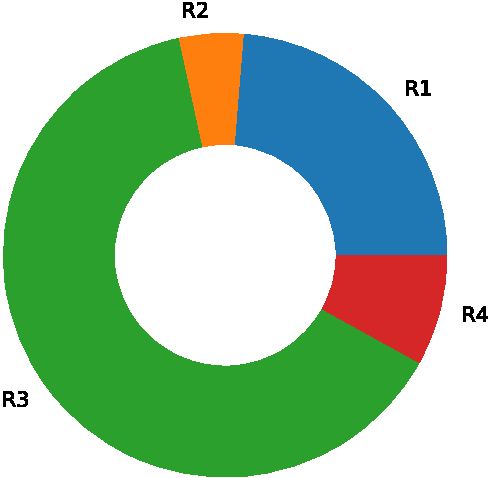
\includegraphics[scale = 0.75]{1.pdf}}
\caption{Моя діаграма ризиків.}
\end{minipage}
\hspace{1cm}
\begin{minipage}[h]{0.5\linewidth}
\center{
\includegraphics[scale = 0.75]{2.pdf}}
\caption{Діаграми ризиків смертельних небезпек будівельника.}
\end{minipage}
\end{figure}
де \xmybox[green]{$R_1$} --- ризик смертельної небезпеки внаслідок соматичних та генетичних
захворювань, а також через природне старіння організму; \xmybox[green]{$R_2$} --- ризик загибелі протягом року внаслідок можливого нещасного випадку на
виробництві; \\ \xmybox[green]{$R_3$} --- ризик наразитися на смертельну небезпеку протягом року внаслідок можливого нещасного випадку в побуті; \xmybox[green]{$R_4$} --- ризик наразитися на смертельну небезпеку протягом року, зумовлений індивідуальним способом життя людини.

\vspace{0.5cm}
\begin{minipage}{0.4\textwidth}
Висновок: сумарний ризик є дуже високим через імовірність утоплення та можливість нещасного випадку в побутi.
\end{minipage}
\hfill
\begin{minipage}{0.4\textwidth}
Висновок: сумарний ризик є дуже високим, загалом через усі факори.
\end{minipage}



%----------------------------------------3
\newpage
\begin{center}ДОДАТОК\end{center}
Програма для обрахунку \textbf{всіх} вихідних данних та побудови кругових діаграм:\\
\lstinputlisting[language = Python]{1.py}
\end{document}
